\chapter*{Anhang A - Der Algorithmus}

The algorithm can be divided in:

\begin{enumerate}
\item Receive the entry.
\item Heavy caterpillar decomposition.
\item Balance the tree.
\item Calculate the shifts.
\item Calculate new coordinates.
\item Lift the graph to a polytope. 
\item Round the graph to grid points.
\end{enumerate}
 

\section*{The Entry of the algorithm}

Given a $3$-connected planar graph and a tree representation of this graph, as shown below.

\begin{center}
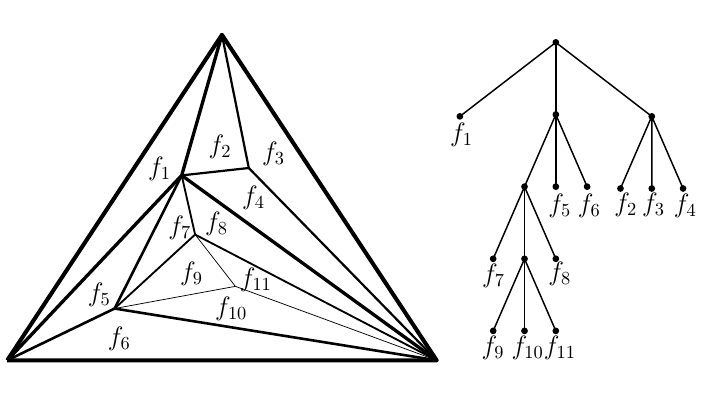
\includegraphics[scale=0.7]{./figures/graph_tree.png} 
\end{center}

\section*{Heavy caterpillar decomposition}
The tree representation is decomposed in \textit{heavy paths}. The resulting sub-trees are called \textit{caterpillars}. If a node lies on a heavy path it is called a \textit{spine node}, otherwise is a \textit{tree node}. The spine nodes are labelled by $s_1$ (root), $s_2$, ..., $s_i$,...,$s_\bot$. The children of $s_i$ are $s_{i+1}$, $t_{i+1}$ and $t'_{i+1}$. We store a pointer link in $t$ to another caterpillar - called $(t)$.

\begin{center}
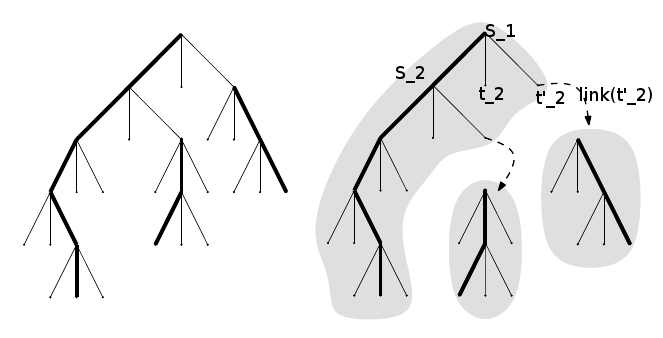
\includegraphics[scale=0.7]{./figures/caterpillarEdit.png} 
\end{center}

\section*{Balance the tree}

The pseudocode below shows the balancing of the tree.

\begin{algorithmic}
\Function{BALANCE}{C} 
\State \textbf{Input:} A caterpillar $C$ from the heavy caterpillar decomposition of $\tau(G)$. All weights are equal 1.
\State \textbf{Output:} Weights for the nodes of $\tau(G)$.

\If {isSmallestFace}
	\State return;
\Else
	\State BALANCE(($s_i$))
	\State BALANCE(link($t_i$))
	\State BALANCE(link($t'_i$))

	\If {$w(t_i)>w(t'_i)$}
        \State relabel $t_i \leftrightarrow t'_i$
	\EndIf

	\State $w(t_i)=w(t'_i)$
	
	\State $w(s_{i-1})$ = $w(s_i) + 2w(t_i)$ 
\EndIf
\EndFunction
\end{algorithmic}
A balanced tree has the following properties:

$$w(s_{i-1})= w(s_i) + w(t_i) + w(t'_i)$$

$$w(s_i)\geq w(t_i),w(t'_i) $$

$$w(t_i)= w(t'_i) $$

An example of a balanced tree is shown in the following graphic: 

\begin{center}
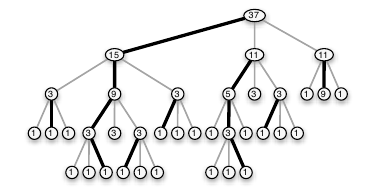
\includegraphics[scale=1]{./figures/balancedTree.png} 
\end{center}

\subsection*{Calculate the shifts} 

After stacking a vertex $v_i$ on a face $f_D$ , we get the new height:

$$z= \zeta_i + z_D $$

Where $z_D$ is the height of the point in the face $D$ and the shift $\zeta_i$ is:

$$\zeta_i = A_i\cdot B_i$$

Where  $ A_i$ and $B_i$ are the two possible weights of the three new faces formed by the vertex $v_i$. Remember $w(t_i)= w(t'_i) $.

But before we calculate the new heights ($z_i$) we round the coordinates in the embedding and the heights.

\subsection*{Calculate new coordinates}

The flat graph needs to have barycentric coordinates. In our case, the areas from the triangle has to be the values of the balanced tree. To calculate the new coordinates we use the formula: $P = t_1\cdot A + t_2\cdot B + t_3\cdot C$, where $t_1$,$t_2$,$t_3$ are proportional to the areas in opposition to the points $A$,$B$,$C$.

\subsection*{Round the graph to grid points}

We have to round the coordinates on the embedding so that they are multiples of $1/\text{pert}$, where:

$$\text{pert}=240R^{\frac{3}{2}}$$

$R$ is the weight of the root from the balanced tree.

Now we lift by rounding the points so that the heights $z= \zeta_i + z_D $ are multiples of $1/\text{pert}_z$, where: 

$$\text{pert}_z=3R$$ 

After these points are rounded they are still real numbers, not integers. To make them integer we multiply them with pert.

To round the coordinate we calculate:

$$\lfloor x\cdot\text{pert}\rfloor \div \text{pert}$$

To gain the final value in integer:

$$\lfloor x\cdot\text{pert}\rfloor \div \text{pert} \cdot\text{pert} = \lfloor x\cdot\text{pert}\rfloor$$